\subsection{Connectedness and Continuity}\label{subsec:connectedness-and-continuity}

Connectedness forbids separated decompositions; continuity transfers local and global topological structure.\\
This subsection develops metric limits, compact-image results, the intermediate value theorem, and paths.

\begin{definition} \label{def:separated-and-connected-sets} \hlt{Separated and Connected Sets}\\
Let $X$ be a metric space.
\begin{enumerate}[label=(\roman*)]
\setlength{\itemsep}{0pt}
\item Subsets $A,B\subseteq X$ are \hlt{separated} iff $A\cap\overline{B}=\overline{A}\cap B=\emptyset$.
\item A subset $E\subseteq X$ is \hlt{connected} iff no nonempty separated $A,B\subseteq E$ satisfy $E=A\cup B$.
\item A subset $U\subseteq X$ is \hlt{clopen} iff it is both open and closed.
\end{enumerate}
\end{definition}

\begin{theorem} \label{thm:connected-subsets-of-real-line-interval-property} \hlt{Connected Subsets of the Real Line}\\
A set $E\subseteq\R$ is connected iff $(\forall x,y\in E)\,[x<y\Longrightarrow[x,y]\subseteq E]$.
\begin{proof}
\begin{enumerate}[label=\roman*.]
\setlength{\itemsep}{0pt}
\item[$(\Rightarrow)$] If the interval property fails, choose $x,y\in E$ and $x<z<y$ with $z\notin E$. Set $A\defeq E\cap(-\infty,z)$ and $B\defeq E\cap(z,\infty)$.\\
Then $A,B\neq\emptyset$ and $E=A\cup B$. The inclusions $\overline{A}\subseteq(-\infty,z]$ and $\overline{B}\subseteq[z,\infty)$ imply $A\cap\overline{B}=\overline{A}\cap B=\emptyset$.\\
Thus $A,B$ separate $E$, contrary to connectedness.
\item[$(\Leftarrow)$] Assume the interval property and suppose $E=A\cup B$ for nonempty separated $A,B$.\\
Choose $x\in A$ and $y\in B$; interchange $A,B$ if necessary so that $x<y$. Set $S\defeq A\cap[x,y]$ and $z\defeq\sup S$.\\
Then $z\in\overline{A}$ by Theorem \ref{thm:supremum-belongs-to-closure}(i). Hence $z\notin B$ by separatedness, and $z<y$ because $y\in B$.\\
If $z\notin A$, then $z\in[x,y]\setminus E$, contrary to the interval property. If $z\in A$, then $z\notin\overline{B}$; choose $r>0$ with $B_r(z)\cap B=\emptyset$.\\
Set $z_1\defeq z+\frac{1}{2}\min\{r,y-z\}$. Then $z<z_1<y$, $z_1\notin B$, and $z_1\notin A$ by $z=\sup S$.\\
Thus $z_1\in[x,y]\setminus E$, again contrary to the interval property.
\end{enumerate}
\hlt{Structural Commentary}: A gap induces a separation; a separation produces a gap at the supremum of one side.\\
\hlt{Key Insight}: The supremum locates the missing boundary point between separated pieces.
\end{proof}
\end{theorem}

\begin{method} \label{meth:compact-connected-proof-patterns} \hlt{Compactness and Connectedness Proof Patterns}
\begin{enumerate}[label=(\roman*)]
\setlength{\itemsep}{0pt}
\item \hlt{Open-cover compactness}: to prove $K$ compact, start with open cover $\{G_\alpha\}_{\alpha\in A}$. Find finite $F\subseteq A$ with $K\subseteq\bigcup\limits_{\alpha\in F}G_\alpha$.
\item \hlt{Euclidean closed-bounded compactness}: to prove a closed bounded set $E\subseteq\R^k$ compact, choose a compact $k$-cell $I\supseteq E$.\\
Then $E$ is compact by Theorem \ref{thm:closed-subsets-of-compact-sets-compact}.
\item \hlt{Connectedness on $\R$}: replace connectedness of $E\subseteq\R$ by $(\forall x,y\in E)\,[x<y\Longrightarrow[x,y]\subseteq E]$.
\end{enumerate}
\end{method}

\begin{definition} \label{def:function-limit-metric} \hlt{Limit of a Function Between Metric Spaces}\\
Let $(X,d_X),(Y,d_Y)$ be metric spaces, let $E\subseteq X$, let $f:E\to Y$, and let $p$ be a limit point of $E$.\\
For $q\in Y$, $\lim\limits_{x\to p}f(x)=q$ iff $(\forall\varepsilon>0)(\exists\delta>0)(\forall x\in E)\,[0<d_X(x,p)<\delta\Longrightarrow d_Y(f(x),q)<\varepsilon]$.\\
The point $p$ need not belong to $E$, and $f(p)$ is irrelevant when it does.\\
\hlt{Key Insight}: A punctured interval determines whether approach is two-sided, right-sided, or left-sided.
\end{definition}

Figure \ref{fig:function-limit-epsilon-delta} illustrates the punctured-neighborhood test in the definition.
\begin{illustrationfigure}[H]
  \centering
  \begin{tikzpicture}[
  scale=0.82,
  >=Stealth,
  every node/.style={font=\scriptsize},
  axis/.style={->, gray!70, line width=0.45pt},
  curve/.style={blue!70!black, line width=0.9pt},
  guide/.style={gray!55, dashed, line width=0.45pt},
  band/.style={orange!12},
  domainband/.style={teal!12, draw=teal!70!black, line width=0.45pt}
]
  \draw[axis] (-0.4,0) -- (7.2,0) node[right] {$x$};
  \draw[axis] (0,-0.35) -- (0,3.75) node[above] {$y$};

  \path[band] (0,1.75) rectangle (6.95,2.85);
  \draw[guide] (0,2.85) -- (6.95,2.85);
  \draw[guide] (0,2.30) -- (6.95,2.30);
  \draw[guide] (0,1.75) -- (6.95,1.75);
  \node[left] at (0,2.85) {$q+\varepsilon$};
  \node[left] at (0,2.30) {$q$};
  \node[left] at (0,1.75) {$q-\varepsilon$};
  \node[orange!70!black, align=center] at (6.55,2.30) {$B_{\varepsilon}(q)$};

  \draw[curve] plot[smooth, tension=0.75] coordinates {
    (0.45,0.78) (1.15,0.93) (1.90,1.26) (2.65,1.90)
    (3.40,2.30) (4.15,2.58) (4.95,2.73) (5.85,2.95) (6.75,3.35)
  };

  \draw[guide] (2.65,0) -- (2.65,1.90);
  \draw[guide] (3.40,0) -- (3.40,2.30);
  \draw[guide] (4.15,0) -- (4.15,2.58);
  \draw[domainband] (2.65,-0.10) rectangle (4.15,0.13);
  \draw[teal!80!black, line width=1.0pt] (2.65,0.08) -- (3.34,0.08);
  \draw[teal!80!black, line width=1.0pt] (3.46,0.08) -- (4.15,0.08);
  \draw[fill=white, draw=teal!80!black, line width=0.7pt] (3.40,0.08) circle (0.055);

  \node[below] at (2.65,-0.10) {$p-\delta$};
  \node[below] at (3.40,-0.10) {$p$};
  \node[below] at (4.15,-0.10) {$p+\delta$};
  \node[teal!70!black, below] at (3.40,-0.45) {punctured $B_{\delta}(p)$};

  \fill[blue!70!black] (3.40,2.30) circle (0.045);
\end{tikzpicture}

  \caption{The epsilon--delta geometry for \(\lim\limits_{x\to p} f(x)=q\).}
  \label{fig:function-limit-epsilon-delta}
\end{illustrationfigure}

\begin{theorem} \label{thm:function-limit-sequential-characterization} \hlt{Sequential Characterization of Function Limits}\\
Let $(X,d_X),(Y,d_Y)$ be metric spaces, let $E\subseteq X$, let $f:E\to Y$, and let $p$ be a limit point of $E$.\\
For $q\in Y$, $\lim\limits_{x\to p}f(x)=q$ iff $f(p_n)\to q$ whenever $(p_n)\subseteq E\setminus\{p\}$ and $p_n\to p$.
\begin{proof}
\begin{enumerate}[label=\roman*.]
\setlength{\itemsep}{0pt}
\item[$(\Rightarrow)$] Let $(p_n)\subseteq E\setminus\{p\}$ satisfy $p_n\to p$, and fix $\varepsilon>0$.\\
Choose $\delta>0$ with $(\forall x\in E)\,[0<d_X(x,p)<\delta\Longrightarrow d_Y(f(x),q)<\varepsilon]$ by Definition \ref{def:function-limit-metric}.\\
Eventually $0<d_X(p_n,p)<\delta$, hence eventually $d_Y(f(p_n),q)<\varepsilon$. Thus $f(p_n)\to q$.
\item[$(\Leftarrow)$] If the limit fails, choose $\varepsilon>0$ with $(\forall\delta>0)(\exists x\in E)\,[0<d_X(x,p)<\delta\land d_Y(f(x),q)\geq\varepsilon]$.\\
Then $p$ is a limit point of $A_\varepsilon\defeq\{x\in E\setminus\{p\}:d_Y(f(x),q)\geq\varepsilon\}$.\\
Choose $(x_n)\subseteq A_\varepsilon$ with $x_n\to p$ by Theorem \ref{thm:metric-sequence-basic-properties}(iii). Since $(\forall n\in\N)\,d_Y(f(x_n),q)\geq\varepsilon$, $f(x_n)\not\to q$.
\end{enumerate}
\hlt{Structural Commentary}: The forward direction transfers a $\delta$-bound; the reverse direction selects from the bad set.\\
\hlt{Key Insight}: Failure of one $\varepsilon$ creates a sequence that defeats convergence.
\end{proof}
\end{theorem}

\begin{corollary} \label{cor:function-limits-are-unique} \hlt{Uniqueness of Function Limits}\\
Let $X,Y$ be metric spaces, $E\subseteq X$, $f:E\to Y$, $p$ be a limit point of $E$. If $f$ has a limit at $p$, then that limit is unique.
\begin{proof}
Let $q$ and $r$ be limits of $f$ at $p$. Choose $(p_n)\subseteq E\setminus\{p\}$ with $p_n\to p$ by Theorem \ref{thm:metric-sequence-basic-properties}(iii).\\
Then $f(p_n)\to q$ and $f(p_n)\to r$ by Theorem \ref{thm:function-limit-sequential-characterization}. Hence $q=r$ by Theorem \ref{thm:metric-sequence-basic-properties}(ii).\\
\hlt{Structural Commentary}: Limit uniqueness is inherited from metric sequence uniqueness.\\
\hlt{Key Insight}: One approaching sequence cannot have two different limits.
\end{proof}
\end{corollary}

\begin{theorem} \label{thm:function-limit-algebra} \hlt{Algebra of Function Limits}\\
Let $X$ be a metric space, $E\subseteq X$, $p$ be a limit point of $E$. For $f,g:E\to\C$, assume $\lim\limits_{x\to p}f(x)=A$ and $\lim\limits_{x\to p}g(x)=B$. Then:
\begin{enumerate}[label=(\roman*)]
\setlength{\itemsep}{0pt}
\item $\lim\limits_{x\to p}(f+g)(x)=A+B$;
\item $\lim\limits_{x\to p}(fg)(x)=AB$;
\item if $B\neq0$, then $\lim\limits_{x\to p;\,g(x)\neq0}\frac{f(x)}{g(x)}=\frac{A}{B}$;
\item Let $u,v:E\to\R^k$, $\lambda\in\R$. Assume $\lim\limits_{x\to p}u(x)=a$, $\lim\limits_{x\to p}v(x)=b$. Then $u+v\to a+b$, $\lambda u\to\lambda a$, and $u\cdot v\to a\cdot b$ as $x\to p$.
\end{enumerate}
\begin{proof}
Let $(p_n)\subseteq E\setminus\{p\}$ satisfy $p_n\to p$. Then $f(p_n)\to A$ and $g(p_n)\to B$ by Theorem \ref{thm:function-limit-sequential-characterization}.
\begin{enumerate}[label=(\roman*)]
\setlength{\itemsep}{0pt}
\item $(f+g)(p_n)\to A+B$ by Theorem \ref{thm:complex-sequence-limit-algebra}(i). Hence (i) by Theorem \ref{thm:function-limit-sequential-characterization}.
\item $(fg)(p_n)\to AB$ by Theorem \ref{thm:complex-sequence-limit-algebra}(iii). Hence (ii) by Theorem \ref{thm:function-limit-sequential-characterization}.
\item Set $U\defeq\{x\in E:g(x)\neq0\}$. Choose $r>0$ with $(\forall x\in E)\,[0<d_X(x,p)<r\Longrightarrow\abs{g(x)-B}<\frac{\abs{B}}{2}]$ by $\lim\limits_{x\to p}g(x)=B$.\\
Then $E\cap B_r(p)\setminus\{p\}\subseteq U$ by the reverse triangle inequality, so $p$ is a limit point of $U$.\\
If $(q_n)\subseteq U\setminus\{p\}$ and $q_n\to p$, then $f(q_n)\to A$ and $g(q_n)\to B$ by Theorem \ref{thm:function-limit-sequential-characterization}.\\
Thus $\frac{f(q_n)}{g(q_n)}\to\frac{A}{B}$ by Theorem \ref{thm:complex-sequence-limit-algebra}(iii),(iv). Hence (iii) by Theorem \ref{thm:function-limit-sequential-characterization}.
\item Under the hypotheses of (iv), $u(p_n)\to a$ and $v(p_n)\to b$ by Theorem \ref{thm:function-limit-sequential-characterization}.\\
Three vector limits hold by Theorem \ref{thm:rk-sequence-coordinate-convergence}(ii)--(iv), with constant scalar sequence $(\lambda)$. Hence (iv) by Theorem \ref{thm:function-limit-sequential-characterization}.
\end{enumerate}
\hlt{Structural Commentary}: Sequential characterization transfers scalar and vector sequence algebra to function limits.\\
\hlt{Key Insight}: Every approaching sequence inherits the corresponding algebraic limit.
\end{proof}
\end{theorem}

\begin{proposition} \label{prop:function-limits-are-local} \hlt{Function Limits Are Local}\\
Let $X,Y$ be metric spaces, $E\subseteq X$, $f:E\to Y$, $p$ be limit point of $E$, $q\in Y$. $(\forall r>0)\,[\lim\limits_{x\to p;\,x\in E}f(x)=q\Longleftrightarrow\lim\limits_{x\to p;\,x\in E\cap B_r(p)}f(x)=q]$.
\begin{proof}
\begin{enumerate}[label=\roman*.]
\setlength{\itemsep}{0pt}
\item[$(\Rightarrow)$] Any $\delta$ witnessing the limit on $E$ witnesses the limit on $E\cap B_r(p)$ by $E\cap B_r(p)\subseteq E$.
\item[$(\Leftarrow)$] Assume the restricted limit and fix $\varepsilon>0$. Choose $\delta_0>0$ by the restricted limit.\\
Then $(\forall x\in E\cap B_r(p))\,[0<d_X(x,p)<\delta_0\Longrightarrow d_Y(f(x),q)<\varepsilon]$. Let $\delta\defeq\min\{\delta_0,r\}$.\\
If $x\in E$ and $0<d_X(x,p)<\delta$, then $x\in E\cap B_r(p)$, so $d_Y(f(x),q)<\varepsilon$.
\end{enumerate}
\hlt{Structural Commentary}: Values away from $p$ cannot affect the limit at $p$.\\
\hlt{Key Insight}: Shrink $\delta$ until every tested point lies in the chosen local neighborhood.
\end{proof}
\end{proposition}

\begin{definition} \label{def:continuity-at-a-point-and-on-a-set} \hlt{Continuity at a Point and on a Set}\\
Let $(X,d_X),(Y,d_Y)$ be metric spaces, $E\subseteq X$, and $f:E\to Y$.
\begin{enumerate}[label=(\roman*)]
\setlength{\itemsep}{0pt}
\item For $p\in E$, $f$ is \hlt{continuous at $p$} iff $(\forall\varepsilon>0)(\exists\delta>0)(\forall x\in E)\,[d_X(x,p)<\delta\Longrightarrow d_Y(f(x),f(p))<\varepsilon]$.
\item The map $f$ is \hlt{continuous on $E$} iff $(\forall p\in E)$, $f$ is continuous at $p$.
\end{enumerate}
\end{definition}

\begin{corollary} \label{cor:maps-continuous-at-isolated-points} \hlt{Every Map Is Continuous at an Isolated Point}\\
Let $(X,d_X),(Y,d_Y)$ be metric spaces, $E\subseteq X$, $f:E\to Y$, $p$ be isolated in $E$. Then $f$ is continuous at $p$.
\begin{proof}
Given $\varepsilon>0$, choose $\delta>0$ with $E\cap B_\delta(p)=\{p\}$. If $x\in E$ and $d_X(x,p)<\delta$, then $x=p$, so $d_Y(f(x),f(p))=0<\varepsilon$.\\
\hlt{Structural Commentary}: Isolation reduces every sufficiently small domain neighborhood to the singleton $\{p\}$.\\
\hlt{Key Insight}: No distinct domain point can approach an isolated point.
\end{proof}
\end{corollary}

\begin{corollary} \label{cor:discrete-domain-maps-continuous} \hlt{Discrete Domains Make Every Map Continuous}\\
Let $X,Y$ be metric spaces, and assume that $X$ carries the discrete metric. Then every map $f:X\to Y$ is continuous.
\begin{proof}
Fix $p\in X$. Then $B_{1/2}(p)=\{p\}$, $p$ isolated; $f$ continuous at $p$ by Corollary \ref{cor:maps-continuous-at-isolated-points}; $f$ continuous on $X$ by Definition \ref{def:continuity-at-a-point-and-on-a-set}(ii).\\
\hlt{Structural Commentary}: In the discrete metric, no distinct point can approach $p$.\\
\hlt{Key Insight}: Pointwise continuity is automatic when small enough balls are singletons.
\end{proof}
\end{corollary}

For the case $E=X$, Figure \ref{fig:metric-continuity-ball-mapping} expresses continuity through nested input and output balls.
\begin{illustrationfigure}[H]
  \centering
  % Source guide: Roman, Advanced Linear Algebra, Ch. 12, Figure 12.2.
% Redrawn schematic for epsilon-delta continuity between metric spaces.
\begin{tikzpicture}[
  >=Stealth,
  every node/.style={font=\small},
  line cap=round,
  line join=round,
  space/.style={draw=gray!60, fill=gray!7, rounded corners=2pt,
    minimum width=2.7cm, minimum height=2.05cm, inner sep=0pt},
  ball/.style={draw=blue!70!black, fill=blue!10, line width=0.65pt},
  imageball/.style={draw=orange!80!black, fill=orange!12, line width=0.65pt},
  imagepatch/.style={draw=teal!70!black, fill=teal!18, line width=0.55pt},
  arrow/.style={->, line width=0.75pt, gray!75},
  point/.style={circle, fill=black, inner sep=1.25pt},
  note/.style={font=\scriptsize, fill=white, inner sep=1.1pt}
]
  \node[space] (X) at (0,0) {};
  \node[space] (Y) at (4.1,0) {};

  \coordinate (x0) at (0,0);
  \coordinate (fx0) at (4.1,0);

  \draw[ball] (x0) circle (0.48);
  \draw[imageball] (fx0) circle (0.78);
  \draw[imagepatch] (fx0) ellipse (0.46 and 0.31);

  \node[point,label={[label distance=2pt]below:$x_0$}] at (x0) {};
  \node[point,label={[label distance=2pt]below:$f(x_0)$}] at (fx0) {};

  \draw[arrow] (X.east) -- node[note, above] {$f$} (Y.west);

  \node[note, anchor=south west] at ([xshift=4pt,yshift=3pt]X.south west) {$X$};
  \node[note, anchor=south west] at ([xshift=4pt,yshift=3pt]Y.south west) {$Y$};
  \node[font=\scriptsize] at (0,0.64) {\textcolor{blue!70!black}{$B_\delta$}};
  \node[font=\scriptsize] at (4.1,0.66) {\textcolor{orange!80!black}{$B_\varepsilon$}};
  \node[font=\scriptsize] at (4.1,0.38) {\textcolor{teal!70!black}{$f(B_\delta)$}};
\end{tikzpicture}

  \caption{Nested balls encode continuity at $x_0$ for $E=X$; adapted from \citet[Ch.~12, Fig.~12.2]{roman2008advanced}.}
  \label{fig:metric-continuity-ball-mapping}
\end{illustrationfigure}

\begin{theorem} \label{thm:continuity-as-limit-at-limit-point} \hlt{Continuity as Equality with the Function Limit}\\
Let $X,Y$ be metric spaces, $E\subseteq X$, $p\in E$, and $f:E\to Y$. If $p$ is a limit point of $E$, then $f$ is continuous at $p$ iff $\lim\limits_{x\to p}f(x)=f(p)$.
\begin{proof}
\begin{enumerate}[label=\roman*.]
\setlength{\itemsep}{0pt}
\item[$(\Rightarrow)$] Fix $\varepsilon>0$, $\delta>0$ by continuity at $p$. If $x\in E$, $0<d_X(x,p)<\delta$, then $d_Y(f(x),f(p))<\varepsilon$. Thus $\lim\limits_{x\to p}f(x)=f(p)$.
\item[$(\Leftarrow)$] Fix $\varepsilon>0$, $\delta>0$ by $\lim\limits_{x\to p}f(x)=f(p)$. If $x\in E\setminus\{p\}$, $d_X(x,p)<\delta$, then $d_Y(f(x),f(p))<\varepsilon$; if $x=p$, distance is $0$.
\end{enumerate}
\hlt{Structural Commentary}: Continuity is the compatibility of the value at $p$ with nearby values.\\
\hlt{Key Insight}: Limits ignore the point; continuity ties the point back in.
\end{proof}
\end{theorem}

\begin{remark} \label{rem:adherent-function-limits-convention} \hlt{Adherent-Point Limit Convention}\\
The adherent-point convention takes $p\in\overline{E}$ and allows $x=p$ in the $\delta$-test.\\
Definition \ref{def:function-limit-metric} instead assumes $p$ is a limit point and requires $0<d_X(x,p)$.\\
If $p\in E$, the unpunctured convention tests $f(p)$ and forces $q=f(p)$.\\
For punctured limits, this condition is continuity at $p$ by Theorem \ref{thm:continuity-as-limit-at-limit-point}.\\
\hlt{Key Insight}: Punctured limits study nearby values; continuity adds compatibility with the value at the point.
\end{remark}

\begin{remark} \label{rem:sequential-continuity-real-line} \hlt{The Sequence-First View}\\
At limit points of a real domain, continuity is equivalent to $x_n\to p\Longrightarrow f(x_n)\to f(p)$.\\
This equivalence holds by Theorems \ref{thm:function-limit-sequential-characterization} and \ref{thm:continuity-as-limit-at-limit-point}. Continuity at isolated points holds by Corollary \ref{cor:maps-continuous-at-isolated-points}.
\end{remark}

\begin{theorem} \label{thm:metric-continuity-sequential-characterization} \hlt{Sequential Characterization of Continuity}\\
Let $(X,d_X),(Y,d_Y)$ be metric spaces, $f:X\to Y$, and $p\in X$. Then $f$ is continuous at $p$ iff $(x_n)\subseteq X$ and $x_n\to p$ imply $f(x_n)\to f(p)$.
\begin{proof}
\begin{enumerate}[label=\roman*.]
\setlength{\itemsep}{0pt}
\item[$(\Rightarrow)$] Assume $f$ is continuous at $p$ and let $x_n\to p$.\\
Given $\varepsilon>0$, choose $\delta>0$ such that $(\forall\,x\in X)\,[d_X(x,p)<\delta\Longrightarrow d_Y(f(x),f(p))<\varepsilon]$.\\
Since $x_n\to p$, eventually $d_X(x_n,p)<\delta$, hence eventually $d_Y(f(x_n),f(p))<\varepsilon$. Thus $f(x_n)\to f(p)$.
\item[$(\Leftarrow)$] Suppose the sequential condition holds and $f$ is not continuous at $p$.\\
Choose $\varepsilon_0>0$ with $(\forall\delta>0)(\exists x\in X)\,[d_X(x,p)<\delta\land d_Y(f(x),f(p))\geq\varepsilon_0]$.\\
Then $p$ is a limit point of $A\defeq\{x\in X:d_Y(f(x),f(p))\geq\varepsilon_0\}$.\\
Choose $(x_n)\subseteq A$ with $x_n\to p$ by Theorem \ref{thm:metric-sequence-basic-properties}(iii). Since $(\forall n\in\N)\,d_Y(f(x_n),f(p))\geq\varepsilon_0$, $f(x_n)\nrightarrow f(p)$, a contradiction.
\end{enumerate}
\hlt{Structural Commentary}: Failure of epsilon--delta continuity manufactures a bad sequence.\\
\hlt{Key Insight}: In metric spaces, sequences detect continuity at points.
\end{proof}
\end{theorem}

\begin{theorem} \label{thm:continuous-composition} \hlt{Composition of Continuous Functions}\\
Let $E\subseteq X$ and let $f:E\to Y$, $g:f(E)\to Z$ be maps between metric spaces.\\
If $f$ is continuous at $p\in E$ and $g$ is continuous at $f(p)$, then $g\circ f$ is continuous at $p$.
\begin{proof}
Given $\varepsilon>0$, choose $\eta>0$ by continuity of $g$ at $f(p)$. Choose $\delta>0$ by continuity of $f$ at $p$ with tolerance $\eta$.\\
If $x\in E$ and $d_X(x,p)<\delta$, then $d_Y(f(x),f(p))<\eta$, hence $d_Z(g(f(x)),g(f(p)))<\varepsilon$.\\
\hlt{Structural Commentary}: The output tolerance for $g$ becomes the input tolerance for $f$.\\
\hlt{Key Insight}: Continuity composes by passing epsilon through an intermediate eta.
\end{proof}
\end{theorem}

\begin{theorem} \label{thm:distance-function-is-continuous} \hlt{The Distance Function Is Continuous}\\
Let $(X,d)$ be a metric space and $D:X\times X\to\R$, $D(x,y)\defeq d(x,y)$.\\
For $d_\times\in\{d_{\mathrm{sum}},d_E,d_{\max}\}$ on $X\times X$, $D:(X\times X,d_\times)\to\R$ is continuous.\\
Equivalently, $x_n\to x$ and $y_n\to y$ in $X$ imply $d(x_n,y_n)\to d(x,y)$.
\begin{proof}
For $x,y,u,v\in X$, $\abs{D(x,y)-D(u,v)}\leq d(x,u)+d(y,v)$ by triangle inequality. Thus $x_n\to x$, $y_n\to y$ imply $D(x_n,y_n)\to D(x,y)$.\\
Convergence under $d_{\mathrm{sum}}$ is equivalent to coordinate convergence because both summands are nonnegative.\\
Continuity for $d_{\mathrm{sum}}$ follows by Theorem \ref{thm:metric-continuity-sequential-characterization}. Other product metrics have same convergent sequences by Proposition \ref{prop:product-metric-comparison}(iii).\\
\hlt{Structural Commentary}: Distance changes continuously when both endpoints move.\\
\hlt{Key Insight}: The triangle inequality controls distance error by endpoint errors.
\end{proof}
\end{theorem}

\begin{theorem} \label{thm:continuity-open-preimages} \hlt{Continuity via Open Preimages}\\
For metric spaces $X,Y$, a map $f:X\to Y$ is continuous iff $f^{-1}(V)$ is open in $X$ whenever $V\subseteq Y$ is open.
\begin{proof}
\begin{enumerate}[label=\roman*.]
\setlength{\itemsep}{0pt}
\item[$(\Rightarrow)$] If $p\in f^{-1}(V)$, $V$ is open, choose $\varepsilon>0$ with $B_\varepsilon(f(p))\subseteq V$. By continuity, $\exists$ $\delta>0$ with $B_\delta(p)\subseteq f^{-1}(V)$, so $f^{-1}(V)$ is open.
\item[$(\Leftarrow)$] For $p\in X$ and $\varepsilon>0$, the ball $V=B_\varepsilon(f(p))$ is open by Theorem \ref{thm:every-neighborhood-open}.\\
Since $p\in f^{-1}(V)$ and $f^{-1}(V)$ is open, some $B_\delta(p)\subseteq f^{-1}(V)$; this is continuity at $p$.
\end{enumerate}
\hlt{Structural Commentary}: Continuity is exactly preservation of openness under inverse image.\\
\hlt{Key Insight}: Images are not Boolean-exact, but preimages are; continuity belongs to preimages.
\end{proof}
\end{theorem}

\begin{proposition} \label{prop:relative-domain-continuity-open-preimages} \hlt{Continuity on a Relative Domain}\\
Let $(X,d_X)$ and $(Y,d_Y)$ be metric spaces, let $E\subseteq X$, and let $f:E\to Y$. The following are equivalent:
\begin{enumerate}[label=(\roman*)]
\setlength{\itemsep}{0pt}
\item $f:(E,d_X|_{E\times E})\to(Y,d_Y)$ is continuous.
\item The set $f^{-1}(V)$ is open relative to $E$ whenever $V\subseteq Y$ is open.
\item If $V\subseteq Y$ is open, then $f^{-1}(V)=E\cap G$ for an open set $G\subseteq X$.
\end{enumerate}
\begin{proof}
Every constant map $h:X\to\R$ is continuous by Definition \ref{def:continuity-at-a-point-and-on-a-set}, since $\abs{h(x)-h(p)}=0$.
\begin{enumerate}[label=(\roman*)]
\setlength{\itemsep}{0pt}
\item[$(i)$]$\Rightarrow (ii)$ For open $V\subseteq Y$, the set $f^{-1}(V)$ is open in the metric space $E$ by Theorem \ref{thm:continuity-open-preimages}.
\item[$(ii)$]$\Rightarrow (iii)$ For open $V\subseteq Y$, choose open $G\subseteq X$ with $f^{-1}(V)=E\cap G$ by Theorem \ref{thm:relative-open-intersection-with-open-set}.
\item[$(iii)$]$\Rightarrow (i)$ For open $V\subseteq Y$, $f^{-1}(V)=E\cap G$ with $G$ open in $X$, hence $f^{-1}(V)$ is open in $E$.\\
Therefore $f$ is continuous by Theorem \ref{thm:continuity-open-preimages} on $E$.
\end{enumerate}
\hlt{Structural Commentary}: Open preimages are relative opens in $E$.\\
\hlt{Key Insight}: Relative continuity says ordinary open sets in $X$ are seen through intersection with $E$.
\end{proof}
\end{proposition}

Figure \ref{fig:continuity-preimage-open} visualizes the inverse-image characterization of continuity.
\begin{illustrationfigure}[H]
  \centering
  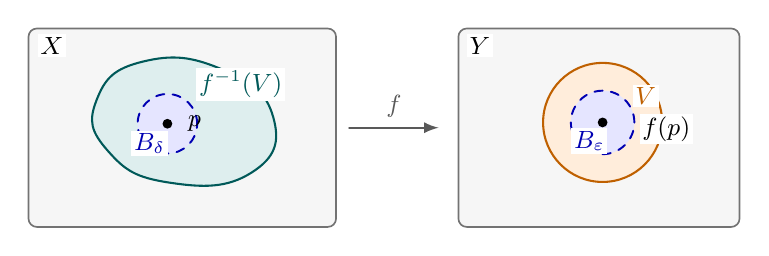
\begin{tikzpicture}[
  scale=0.84,
  >=latex,
  every node/.style={font=\small},
  line cap=round,
  line join=round,
  ambient/.style={draw=black!55, fill=gray!7, rounded corners=3pt, line width=0.6pt},
  preimage/.style={draw=teal!70!black, fill=teal!13, line width=0.75pt},
  openrange/.style={draw=orange!75!black, fill=orange!14, line width=0.75pt},
  ball/.style={draw=blue!70!black, fill=blue!10, dashed, line width=0.7pt},
  arrow/.style={->, black!65, line width=0.8pt},
  point/.style={circle, fill=black, inner sep=1.25pt},
  note/.style={fill=white, inner sep=1pt}
]
  \begin{scope}
    \draw[ambient] (-2.65,-1.5) rectangle (2.0,1.5);
    \node[note, anchor=north west] at (-2.52,1.42) {$X$};
    \draw[preimage]
      plot[smooth cycle, tension=0.85] coordinates {
        (-1.62,0.42) (-0.92,1.0) (0.28,0.88) (1.05,0.16)
        (0.72,-0.68) (-0.52,-0.83) (-1.45,-0.35)
      };
    \coordinate (p) at (-0.55,0.06);
    \draw[ball] (p) circle (0.45);
    \node[point,label={[label distance=2pt]right:$p$}] at (p) {};
    \node[teal!70!black, note, anchor=center] at (0.56,0.66) {$f^{-1}(V)$};
    \node[blue!70!black, note, anchor=center] at (-0.82,-0.24) {$B_\delta$};
  \end{scope}

  \begin{scope}[xshift=5.55cm]
    \draw[ambient] (-1.7,-1.5) rectangle (2.55,1.5);
    \node[note, anchor=north west] at (-1.58,1.42) {$Y$};
    \draw[openrange] (0.48,0.08) circle (0.9);
    \draw[ball] (0.48,0.08) circle (0.48);
    \node[point] at (0.48,0.08) {};
    \node[note, anchor=west] at (1.03,-0.02) {$f(p)$};
    \node[orange!75!black, note, anchor=center] at (1.13,0.48) {$V$};
    \node[blue!70!black, note, anchor=center] at (0.28,-0.20) {$B_\varepsilon$};
  \end{scope}

  \draw[arrow] (2.2,0) -- (3.55,0) node[midway, above] {$f$};
\end{tikzpicture}

  \caption{Continuity pulls open sets back to open sets.}
  \label{fig:continuity-preimage-open}
\end{illustrationfigure}

\begin{corollary} \label{cor:continuity-closed-preimages} \hlt{Continuity via Closed Preimages}\\
Let $X,Y$ be metric spaces, $f:X\to Y$. Then $f$ is continuous iff $f^{-1}(C)$ is closed in $X$ whenever $C\subseteq Y$ is closed.
\begin{proof}
\begin{enumerate}[label=\roman*.]
\setlength{\itemsep}{0pt}
\item[$(\Rightarrow)$] For closed $C\subseteq Y$, $X\setminus f^{-1}(C)=f^{-1}(Y\setminus C)$ is open by Theorem \ref{thm:continuity-open-preimages}. Hence $f^{-1}(C)$ is closed.
\item[$(\Leftarrow)$] For open $V\subseteq Y$, $X\setminus f^{-1}(V)=f^{-1}(Y\setminus V)$ is closed by hypothesis; hence $f^{-1}(V)$ is open.
\end{enumerate}
\hlt{Structural Commentary}: Closed-set continuity is the complement form of open-set continuity.\\
\hlt{Key Insight}: $f^{-1}(Y\setminus C)=X\setminus f^{-1}(C)$ transfers open and closed formulations.
\end{proof}
\end{corollary}

\begin{perspective} \label{per:three-views-of-continuity} \hlt{Three Views of Continuity}\\
For metric-space maps, continuity has three equivalent forms: $\varepsilon$--$\delta$ control, sequence preservation, and open inverse images.\\
The owners are Definition \ref{def:continuity-at-a-point-and-on-a-set} and Theorems \ref{thm:metric-continuity-sequential-characterization}, \ref{thm:continuity-open-preimages}.\\
\hlt{Key Insight}: Continuity sends near points forward and pulls open sets back.
\end{perspective}

\begin{proposition} \label{prop:distance-to-set-is-continuous} \hlt{Distance-to-Set Is Continuous}\\
Let $(X,d)$ be a metric space, let $\emptyset\neq E\subseteq X$, and define $f:X\to\R$ by $f(p)\defeq\operatorname{dist}(p,E)$.
\begin{enumerate}[label=(\roman*)]
\setlength{\itemsep}{0pt}
\item $f$ is $1$-Lipschitz: $(\forall\,p,q\in X)\ \abs{f(p)-f(q)}\leq d(p,q)$.
\item The map $f$ is continuous.
\item $f^{-1}(\{0\})=\overline{E}$.
\end{enumerate}
\begin{proof}
\begin{enumerate}[label=(\roman*)]
\setlength{\itemsep}{0pt}
\item For $p,q\in X$ and $e\in E$, $d(p,e)\leq d(p,q)+d(q,e)$. Then $f(p)-f(q)\leq d(p,q)$ by taking $\inf\limits_{e\in E}$.\\
Interchanging $p,q$, $f(q)-f(p)\leq d(p,q)$. Thus $\abs{f(p)-f(q)}\leq d(p,q)$.
\item Fix $p\in X$ and $\varepsilon>0$, and set $\delta\defeq\varepsilon$. If $d(p,q)<\delta$, then $\abs{f(p)-f(q)}<\varepsilon$ by (i). Hence $f$ is continuous on $X$.
\item For $p\in X$, $p\in f^{-1}(\{0\})$ iff $\operatorname{dist}(p,E)=0$ iff $p\in\overline{E}$ by Proposition \ref{prop:set-distance-closure-criterion}.
\end{enumerate}
\hlt{Structural Commentary}: Distance to a fixed set changes no faster than the point itself moves.\\
\hlt{Key Insight}: The triangle inequality turns nearest-set distance into a continuous detector of closure.
\end{proof}
\end{proposition}

\begin{corollary} \label{cor:open-closed-sets-by-continuous-real-functions} \hlt{Open and Closed Sets by Distance Functions}\\
Let $X$ be a metric space.
\begin{enumerate}[label=(\roman*)]
\setlength{\itemsep}{0pt}
\item A set $O\subseteq X$ is open iff $O=\{x\in X:f(x)>0\}$ for a continuous map $f:X\to\R$.
\item A set $F\subseteq X$ is closed iff $F=g^{-1}(\{0\})$ for a continuous map $g:X\to\R$.
\end{enumerate}
\begin{proof}
\begin{enumerate}[label=(\roman*)]
\setlength{\itemsep}{0pt}
\item[$(i)$] ($\Rightarrow$) If $O=X$, take $f\equiv1$; this map is continuous and $O=\{x\in X:f(x)>0\}$.\\
If $O\neq X$, set $f(x)\defeq\operatorname{dist}(x,O^c)$. Then $f$ is continuous by Proposition \ref{prop:distance-to-set-is-continuous}(ii).\\
Since $O^c$ is closed, $f^{-1}(\{0\})=O^c$ by Proposition \ref{prop:distance-to-set-is-continuous}(iii). Hence $O=\{x\in X:f(x)>0\}$.
\item[$(i)$] ($\Leftarrow$) If $O=\{x\in X:f(x)>0\}$ for continuous $f:X\to\R$, then $O=f^{-1}((0,\infty))$ is open by Theorem \ref{thm:continuity-open-preimages}.
\item[$(ii)$] ($\Rightarrow$) If $F=\emptyset$, take $g\equiv1$; this map is continuous and $F=g^{-1}(\{0\})$. If $F\neq\emptyset$, set $g(x)\defeq\operatorname{dist}(x,F)$.\\
Then $g$ is continuous by Proposition \ref{prop:distance-to-set-is-continuous}(ii). Since $F$ is closed, $g^{-1}(\{0\})=\overline{F}=F$ by Proposition \ref{prop:distance-to-set-is-continuous}(iii).
\item[$(ii)$] ($\Leftarrow$) If $F=g^{-1}(\{0\})$ for a continuous $g:X\to\R$, then $F$ is closed by Corollary \ref{cor:continuity-closed-preimages}.
\end{enumerate}
\hlt{Structural Commentary}: Metric spaces encode open and closed sets by continuous real-valued distance functions.\\
\hlt{Key Insight}: A set is closed exactly when its distance-zero locus has no extra points.
\end{proof}
\end{corollary}

\begin{definition} \label{def:homeomorphism} \hlt{Homeomorphism}\\
Let $X$, $Y$ be metric spaces. A \hlt{homeomorphism} from $X$ to $Y$ is a bijection $f:X\to Y$ such that both $f$ and $f^{-1}$ are continuous.\\
If such a map exists, $X$ and $Y$ are \hlt{homeomorphic}, written $X\simeq Y$.
\end{definition}

\begin{proposition} \label{prop:homeomorphisms-preserve-topology} \hlt{Homeomorphisms Preserve Topology}\\
If $f:X\to Y$ is a homeomorphism, then $U\mapsto f(U)$ bijects open subsets of $X$ with open subsets of $Y$.
\begin{proof}
If $U\subseteq X$ is open, then $f(U)=(f^{-1})^{-1}(U)$ is open in $Y$ by continuity of $f^{-1}$.\\
If $V\subseteq Y$ is open, then $f^{-1}(V)$ is open in $X$ by continuity of $f$. These assignments are inverse because $f$ is bijective.\\
\hlt{Structural Commentary}: A homeomorphism preserves open sets in both directions.\\
\hlt{Key Insight}: Topological sameness is continuity plus continuous reversibility.
\end{proof}
\end{proposition}

\begin{theorem} \label{thm:metric-isometry-basic-properties} \hlt{Basic Properties of Metric Isometries}\\
Let $f:(X,d_X)\to(Y,d_Y)$ be an isometry.
\begin{enumerate}[label=(\roman*)]
\setlength{\itemsep}{0pt}
\item $f$ is injective.
\item $f$ is continuous.
\item $f^{-1}:(f(X),d_Y|_{f(X)\times f(X)})\to(X,d_X)$ is an isometry.
\end{enumerate}
\begin{proof}
\begin{enumerate}[label=(\roman*)]
\setlength{\itemsep}{0pt}
\item If $f(x)=f(y)$, then $d_X(x,y)=d_Y(f(x),f(y))=0$, hence $x=y$.
\item If $x_n\to x$ in $X$, then $d_Y(f(x_n),f(x))=d_X(x_n,x)\to0$. Hence $f$ is continuous by Theorem \ref{thm:metric-continuity-sequential-characterization}.
\item For $u=f(x),v=f(y)\in f(X)$, $d_X(f^{-1}(u),f^{-1}(v))=d_X(x,y)=d_Y(f(x),f(y))=d_Y(u,v)$.
\end{enumerate}
\hlt{Structural Commentary}: An isometry preserves all distances, so injectivity and continuity are automatic.\\
\hlt{Key Insight}: Distance preservation is stronger than topological equivalence.
\end{proof}
\end{theorem}

\begin{remark} \label{rem:metric-versus-linear-isometries} \hlt{Metric Versus Linear Isometries}\\
Metric isometry is purely distance-theoretic. If $T:V\to W$ is linear between inner-product spaces, then\\
$(\forall v\in V)\,\norm{Tv}=\norm v\Longleftrightarrow(\forall u,v\in V)\,d_W(Tu,Tv)=d_V(u,v)$.
\end{remark}

\begin{counterexample} \label{cex:circle-param-continuous-bijection-not-homeomorphism} \hlt{Continuous Bijection Need Not Be a Homeomorphism}\\
Let $S^1\defeq\{(x,y)\in\R^2:x^2+y^2=1\}$ and define $f:[0,2\pi)\to S^1$ by $f(t)\defeq(\cos t,\sin t)$.\\
This standard parametrization is a continuous bijection. Set $t_n\defeq 2\pi-\frac{1}{n}$ and $z_n\defeq f(t_n)$.\\
Then $z_n\to(1,0)=f(0)$, while $f^{-1}(z_n)=t_n\to2\pi\neq0=f^{-1}(1,0)$.\\
Thus $f^{-1}$ is not continuous by Theorem \ref{thm:metric-continuity-sequential-characterization}, so $f$ is not a homeomorphism.
\end{counterexample}

Figure \ref{fig:circle-interval-wrap-not-homeomorphism} shows the discontinuity created by cutting the circle at one point.
\begin{illustrationfigure}[H]
  \centering
  \begin{tikzpicture}[
  scale=1.0,
  line cap=round,
  line join=round,
  maparrow/.style={->, thick, green!50!black},
  endpoint/.style={orange!85!black},
  purplepoint/.style={purple!70!black},
  point/.style={fill=black, inner sep=0pt}
]
  \coordinate (L) at (-3.25,0);
  \coordinate (R) at (0.55,0);
  \coordinate (C) at (3.55,0);
  \def\r{0.82}
  \coordinate (A) at ($(R)+(0.34,0)$);
  \coordinate (B) at ($(C)+(-\r-0.22,0)$);

  \draw[thick] (L) -- (R);
  \draw[thick] ($(L)+(0,-0.13)$) -- ($(L)+(0,0.13)$);
  \draw[thick, endpoint] ($(R)+(0,0.13)$) arc[start angle=90,end angle=-90,radius=0.13];
  \node[below] at ($(L)+(0,-0.04)$) {$0$};
  \node[endpoint, below] at ($(R)+(0,-0.04)$) {$2\pi$};
  \fill[purplepoint] (-0.12,0) circle (1.4pt);
  \node[purplepoint, above] at (-0.28,0.10) {$f^{-1}(z_n)$};

  \draw[thick] (C) circle (\r);
  \node[above] at ($(C)+(0,\r+0.12)$) {$S^1$};
  \fill[endpoint] ($(C)+(\r,0)$) circle (1.4pt);
  \node[endpoint, right] at ($(C)+(\r+0.08,0.03)$) {$p=(1,0)$};
  \foreach \a in {-38,-31,-25} {
    \fill[purplepoint] ($(C)+({\r*cos(\a)},{\r*sin(\a)})$) circle (1.1pt);
  }
  \node[purplepoint, below right] at ($(C)+({\r*cos(-32)},{\r*sin(-32)})$) {$z_n$};

  \draw[maparrow] (A) -- (B);
  \node[green!50!black, above] at ($(A)!0.5!(B)$) {$f$};
\end{tikzpicture}

  \caption{Parametrization $[0,2\pi)\to S^1$ wraps continuously and bijectively, but inverse jumps at $(1,0)$.}
  \label{fig:circle-interval-wrap-not-homeomorphism}
\end{illustrationfigure}

\begin{remark} \label{rem:continuity-domain-only} \hlt{Continuity Only Uses the Domain Metric}\\
For $f:E\to Y$ with $E\subseteq X$, continuity on $E$ depends only on the restricted metric on $E$, not on $X\setminus E$.
\end{remark}

\begin{definition} \label{def:product-map-direct-sum} \hlt{Product Map}\\
If $f:X\to Y$ and $g:X\to Z$ are maps between metric spaces, their \hlt{product map}, or direct sum, is $f\oplus g:X\to Y\times Z$.\\
It is defined by $(f\oplus g)(x)\defeq(f(x),g(x))$. The product $Y\times Z$ carries any product metric from Definition \ref{def:product-metrics}.
\end{definition}

\begin{proposition} \label{prop:product-map-continuity} \hlt{Continuity of Product Maps}\\
Let $X,Y,Z$ be metric spaces, let $f:X\to Y$, let $g:X\to Z$, and let $x_0\in X$.
\begin{enumerate}[label=(\roman*)]
\setlength{\itemsep}{0pt}
\item The product map $f\oplus g:X\to Y\times Z$ is continuous at $x_0$ iff $f$ and $g$ are continuous at $x_0$.
\item The map $f\oplus g$ is continuous on $X$ iff both $f$ and $g$ are continuous on $X$.
\end{enumerate}
\begin{proof}
By Proposition \ref{prop:product-metric-comparison}(iii), it suffices to use $d_{\mathrm{sum}}$.
\begin{enumerate}[label=(\roman*)]
\setlength{\itemsep}{0pt}
\item[$(i)$] ($\Rightarrow$) Given $\varepsilon>0$, choose $\delta>0$ from continuity of $f\oplus g$ at $x_0$.\\
If $d_X(x,x_0)<\delta$, then $d_Y(f(x),f(x_0)),d_Z(g(x),g(x_0))\leq d_{\mathrm{sum}}((f\oplus g)(x),(f\oplus g)(x_0))<\varepsilon$.
\item[$(i)$] ($\Leftarrow$) Given $\varepsilon>0$, choose $\delta_f,\delta_g$ for $f,g$ at tolerance $\frac{\varepsilon}{2}$. Set $\delta\defeq\min\{\delta_f,\delta_g\}$.\\
If $d_X(x,x_0)<\delta$, then $d_{\mathrm{sum}}((f\oplus g)(x),(f\oplus g)(x_0))=d_Y(f(x),f(x_0))+d_Z(g(x),g(x_0))<\varepsilon$.
\item[$(ii)$] ($\Rightarrow$) If $f\oplus g$ is continuous on $X$, then $(\forall x_0\in X)$, both $f$ and $g$ are continuous at $x_0$ by (i).\\
Hence both are continuous on $X$ by Definition \ref{def:continuity-at-a-point-and-on-a-set}(ii).
\item[$(ii)$] ($\Leftarrow$) If $f$ and $g$ are continuous on $X$, then $(\forall x_0\in X)$, $f\oplus g$ is continuous at $x_0$ by (i).\\
Hence $f\oplus g$ is continuous on $X$ by Definition \ref{def:continuity-at-a-point-and-on-a-set}(ii).
\end{enumerate}
\hlt{Structural Commentary}: Product continuity is exactly componentwise continuity.\\
\hlt{Key Insight}: A product metric packages two output estimates into one.
\end{proof}
\end{proposition}

\begin{theorem} \label{thm:continuous-algebra-and-components} \hlt{Continuous Algebra and Components}\\
Let $X$ be a metric space.
\begin{enumerate}[label=(\roman*)]
\setlength{\itemsep}{0pt}
\item If $f,g:X\to\C$ are continuous, then $f+g$ and $fg$ are continuous on $X$, while $f/g$ is continuous on $U\defeq\{x\in X:g(x)\neq0\}$.
\item For $f=(f_1,\ldots,f_k):X\to\R^k$, $f$ is continuous iff $(\forall j\in\{1,\ldots,k\})\,f_j$ is continuous.
\item If $f,g:X\to\R^k$ are continuous, so are $f+g$ and $f\cdot g$.
\end{enumerate}
\begin{proof}
\begin{enumerate}[label=(\roman*)]
\setlength{\itemsep}{0pt}
\item[$(i)$] If $x_n\to x$ in $X$, then $f(x_n)\to f(x)$ and $g(x_n)\to g(x)$ by Theorem \ref{thm:metric-continuity-sequential-characterization}.\\
Thus $(f+g)(x_n)\to(f+g)(x)$ and $(fg)(x_n)\to(fg)(x)$ by Theorem \ref{thm:complex-sequence-limit-algebra}(i),(iii).\\
If $x\in U$ and $(x_n)\subseteq U$, then $(f/g)(x_n)\to(f/g)(x)$ by Theorem \ref{thm:complex-sequence-limit-algebra}(iii),(iv).\\
The three continuity conclusions follow by Theorem \ref{thm:metric-continuity-sequential-characterization}.
\item[$(ii)$] ($\Rightarrow$) If $f$ is continuous and $x_n\to x$, then $f(x_n)\to f(x)$ by Theorem \ref{thm:metric-continuity-sequential-characterization}.\\
Hence $(\forall j\in\{1,\ldots,k\})\,f_j(x_n)\to f_j(x)$ by Theorem \ref{thm:rk-sequence-coordinate-convergence}(i), so each $f_j$ is continuous.
\item[$(ii)$] ($\Leftarrow$) If each $f_j$ is continuous and $x_n\to x$, then $(\forall j\in\{1,\ldots,k\})\,f_j(x_n)\to f_j(x)$.\\
Hence $f(x_n)\to f(x)$ by Theorem \ref{thm:rk-sequence-coordinate-convergence}(i), so $f$ is continuous.
\item[$(iii)$] Each coordinate of $f+g$ is continuous by (i), so $f+g$ is continuous by (ii).\\
The map $f\cdot g=\sum\limits_{j=1}^k f_jg_j$ is continuous by repeated scalar sums and products in (i).
\end{enumerate}
\hlt{Structural Commentary}: Continuity is stable under the algebraic operations already stable for limits.\\
\hlt{Key Insight}: Componentwise control is equivalent to Euclidean control in finite dimensions.
\end{proof}
\end{theorem}

\begin{theorem} \label{thm:baire-local-uniform-boundedness-continuous-family} \hlt{Pointwise Bounded Families Are Locally Uniformly Bounded}\\
Let $(X,d)$ be a nonempty complete metric space, $\mathcal{F}$ be a family of continuous maps $f:X\to\R$.\\
Assume $(\forall\,x\in X)(\exists\,M_x>0)(\forall\,f\in\mathcal{F})\ \abs{f(x)}\leq M_x$.\\
Then there are a nonempty open set $O\subseteq X$ and $M>0$ such that $(\forall\,x\in O)(\forall\,f\in\mathcal{F})\ \abs{f(x)}\leq M$.
\begin{proof}
For $n\in\N$, set $E_n\defeq\{x\in X:(\forall f\in\mathcal{F})\,\abs{f(x)}\leq n\}$. The interval $[-n,n]=\overline{B}_n(0)$ is closed by Corollary \ref{cor:closed-balls-are-closed}.\\
Hence $E_n=\bigcap\limits_{f\in\mathcal{F}}f^{-1}([-n,n])$ closed by Corollary \ref{cor:continuity-closed-preimages}, Theorem \ref{thm:metric-open-closed-set-calculus}(ii). $X=\bigcup\limits_{n=1}^{\infty}E_n$ by pointwise bound, Theorem \ref{thm:archimedean-and-rational-density}(i).\\
Choose $N\in\N$ with $E_N^\circ\neq\emptyset$ by Corollary \ref{cor:baire-closed-cover-has-interior}(ii). Set $O\defeq E_N^\circ$ and $M\defeq N$. Then $(\forall\,x\in O)(\forall\,f\in\mathcal{F})\ \abs{f(x)}\leq M$.\\
\hlt{Structural Commentary}: Closed inverse images form a countable cover, and Baire supplies one member with interior.\\
\hlt{Key Insight}: One interior level set bounds the entire family locally.
\end{proof}
\end{theorem}

\begin{theorem} \label{thm:pointwise-limit-continuous-on-dense-set} \hlt{Dense Continuity Set for Pointwise Limits}\\
Let $(X,d)$ be a complete metric space, let $f:X\to\R$, and let $(f_n)_{n\in\N}$ be continuous maps $X\to\R$.\\
Assume $(\forall x\in X)\,f_n(x)\to f(x)$. Then $(\exists D\subseteq X)$ satisfying:
\begin{enumerate}[label=(\roman*)]
\setlength{\itemsep}{0pt}
\item $D$ is dense in $X$;
\item $(\forall x_0\in D)(\forall\varepsilon>0)(\exists\delta>0)(\forall n\in\N)(\forall x\in X)\,[d(x,x_0)<\delta\Longrightarrow\abs{f_n(x)-f_n(x_0)}<\varepsilon]$;
\item $(\forall x_0\in D)$, $f$ is continuous at $x_0$.
\end{enumerate}
\begin{proof}
For $m,n\in\N$, set $I_m\defeq[-m^{-1},m^{-1}]$ and $E_{m,n}\defeq\{x\in X:(\forall j,k\geq n)\,f_j(x)-f_k(x)\in I_m\}$.\\
For $j,k\geq n$, the map $f_j-f_k$ is continuous by Theorem \ref{thm:continuous-algebra-and-components}(i). The interval $I_m$ is closed by Corollary \ref{cor:closed-balls-are-closed}.\\
Thus $E_{m,n}=\bigcap\limits_{j,k\geq n}(f_j-f_k)^{-1}(I_m)$ is closed by Corollary \ref{cor:continuity-closed-preimages} and Theorem \ref{thm:metric-open-closed-set-calculus}(ii). Fix $m\in\N$ and $x\in X$.\\
Then $(f_n(x))$ is Cauchy by Theorem \ref{thm:cauchy-convergence-criterion}(i). Choose $N\in\N$ with $x\in E_{m,N}$ by Definition \ref{def:cauchy-sequence}. Hence $X=\bigcup\limits_{n=1}^{\infty}E_{m,n}$.\\
For $E\subseteq X$, $\operatorname{bd}(E)=\overline{E}\cap\overline{E^c}$ by Definitions \ref{def:adherent-points-and-closure} and \ref{def:interior-closure-boundary}(iii). Thus $\operatorname{bd}(E)$ is closed by Theorem \ref{thm:closure-smallest-closed-containing-set}(i) and Theorem \ref{thm:metric-open-closed-set-calculus}(ii).\\
If $E$ closed, $O$ open with $O\subseteq\operatorname{bd}(E)=E\setminus E^\circ$, then $O\subseteq E$. Hence $O\subseteq E^\circ$ by Definition \ref{def:interior-closure-boundary}(i), assumed inclusion forces $O=\emptyset$.\\
Hence boundary of closed set is nowhere dense by Definition \ref{def:fsigma-gdelta-nowhere-dense}(iii). Hence $X\setminus\operatorname{bd}(E_{m,n})$ is dense and open.\\
Set $D\defeq X\setminus\bigcup\limits_{m,n\in\N}\operatorname{bd}(E_{m,n})$. Then $D=\bigcap\limits_{m,n\in\N}\bigl(X\setminus\operatorname{bd}(E_{m,n})\bigr)$ by Theorem \ref{thm:indexed-de-morgan-laws}.
\begin{enumerate}[label=(\roman*)]
\setlength{\itemsep}{0pt}
\item[$(i)$] The set $\N^2$ is countable by Corollary \ref{cor:countable-cartesian-products}(ii). Hence $D$ is dense in $X$ by Theorem \ref{thm:dense-open-baire-complete-metric-space}.
\item[$(ii)$] Fix $x_0\in D$, $\varepsilon>0$. Choose $m\in\N$ with $\frac{3}{m}<\varepsilon$ by Theorem \ref{thm:archimedean-and-rational-density}(i). Choose $N\in\N$ with $x_0\in E_{m,N}$ by $X=\bigcup\limits_{n=1}^{\infty}E_{m,n}$.\\
Since $x_0\notin\operatorname{bd}(E_{m,N})$, $x_0\in E_{m,N}^\circ$; choose $r>0$ with $B_r(x_0)\subseteq E_{m,N}$.\\
For $1\leq i\leq N$, choose $\delta_i>0$ by continuity of $f_i$ at $x_0$ with tolerance $\frac{1}{m}$.\\
Set $\delta\defeq\min\{r,\delta_1,\ldots,\delta_N\}>0$. If $d(x,x_0)<\delta$ and $j>N$, then $x,x_0\in E_{m,N}$.\\
By the triangle inequality, $\abs{f_j(x)-f_j(x_0)}\leq\abs{f_j(x)-f_N(x)}+\abs{f_N(x)-f_N(x_0)}+\abs{f_N(x_0)-f_j(x_0)}$.\\
The three terms are bounded by $m^{-1},m^{-1},m^{-1}$, with the middle bound strict; hence $\abs{f_j(x)-f_j(x_0)}<\frac{3}{m}<\varepsilon$.\\
The same bound holds for $1\leq j\leq N$ by the choice of $\delta$. Hence (ii).
\item[$(iii)$] Fix $x_0\in D$, $\varepsilon>0$, $\eta\defeq\frac{\varepsilon}{2}$. By (ii), choose $\delta>0$ with $(\forall n\in\N)(\forall x\in X)\,[d(x,x_0)<\delta\Longrightarrow\abs{f_n(x)-f_n(x_0)}<\eta]$.\\
If $d(x,x_0)<\delta$, then $f_n(x)-f_n(x_0)\to f(x)-f(x_0)$ by Theorem \ref{thm:complex-sequence-limit-algebra}(i),(ii).\\
Hence $\abs{f_n(x)-f_n(x_0)}\to\abs{f(x)-f(x_0)}$ by reverse triangle inequality; $\abs{f(x)-f(x_0)}\leq\eta<\varepsilon$ by Proposition \ref{prop:convergent-sequence-basic-consequences}(iii).
\end{enumerate}
\hlt{Structural Commentary}: Baire avoids every tail-Cauchy boundary; one interior tail set controls all indices.\\
\hlt{Key Insight}: Tail Cauchy bounds plus finitely many continuous terms create equicontinuity.
\end{proof}
\end{theorem}

\begin{example} \label{ex:coordinate-polynomial-rational-norm-continuity} \hlt{Coordinate, Polynomial, Rational, and Norm Maps}\\
Coordinate maps on $\R^k$ are continuous; hence polynomials are continuous, and rational functions are continuous where defined.\\
The reverse triangle inequality is $\abs{\norm{\mathbf{x}}_2-\norm{\mathbf{y}}_2}\leq\norm{\mathbf{x}-\mathbf{y}}_2$. Hence $\mathbf{x}\mapsto\norm{\mathbf{x}}_2$ is continuous by Definition \ref{def:continuity-at-a-point-and-on-a-set}.\\
Thus $p\mapsto\norm{f(p)}_2$ is continuous for continuous $f:X\to\R^k$ by Theorem \ref{thm:continuous-composition}.
\end{example}

\begin{definition} \label{def:bounded-mapping-into-rk} \hlt{Bounded Mapping}\\
A mapping $f:E\to\R^k$ is \hlt{bounded} iff $(\exists M\in\R)(\forall x\in E)\,\norm{f(x)}_2\leq M$.
\end{definition}

\begin{theorem} \label{thm:continuous-image-compact} \hlt{Continuous Images of Compact Sets Are Compact}\\
Let $X$ and $Y$ be metric spaces. If $f:X\to Y$ is continuous and $X$ is compact, then $f(X)$ is compact.
\begin{proof}
Let $\{V_\alpha\}$ be an open cover of $f(X)$. Then $\{f^{-1}(V_\alpha)\}$ is an open cover of $X$ by Theorem \ref{thm:continuity-open-preimages}.\\
Choose $\alpha_1,\ldots,\alpha_n$ with $X\subseteq\bigcup\limits_{i=1}^n f^{-1}(V_{\alpha_i})$; then $f(X)\subseteq\bigcup\limits_{i=1}^n V_{\alpha_i}$.\\
\hlt{Structural Commentary}: Pull back, take a finite subcover, push forward.\\
\hlt{Key Insight}: Compactness is preserved by continuous images because inverse images preserve openness.
\end{proof}
\end{theorem}

\begin{corollary} \label{cor:continuous-rk-image-compact-closed-bounded} \hlt{Continuous Images into $\R^k$ Are Closed and Bounded}\\
Let $X$ be a metric space. If $f:X\to\R^k$ is continuous, $X$ is compact, then $f(X)$ is closed and bounded; consequently, $f$ is bounded.
\begin{proof}
By Theorem \ref{thm:continuous-image-compact}, $f(X)$ is compact. By Theorem \ref{thm:heine-borel-rk}, compact subsets of $\R^k$ are closed and bounded; hence $f$ is bounded.\\
\hlt{Structural Commentary}: Compactness in the domain becomes closed-bounded geometry in Euclidean range.\\
\hlt{Key Insight}: Continuous functions on compact spaces cannot escape to infinity.
\end{proof}
\end{corollary}

\begin{theorem} \label{thm:extreme-value-theorem-compact} \hlt{Extreme Value Theorem}\\
Let $X$ be a nonempty compact metric space and let $f:X\to\R$ be continuous.\\
If $M\defeq\sup\limits_{p\in X}f(p)$ and $m\defeq\inf\limits_{p\in X}f(p)$, then $(\exists p,q\in X)\,[f(p)=M\land f(q)=m]$.
\begin{proof}
By Corollary \ref{cor:continuous-rk-image-compact-closed-bounded}, $f(X)$ is nonempty, closed, and bounded in $\R$. By Theorem \ref{thm:supremum-belongs-to-closure}(ii), $M=\sup f(X)$ belongs to $f(X)$.\\
Fix $\varepsilon>0$. Since $m+\varepsilon$ is not a lower bound for $f(X)$, choose $y_\varepsilon\in f(X)$ with $m\leq y_\varepsilon<m+\varepsilon$.\\
Hence $m\in\overline{f(X)}=f(X)$. Thus $(\exists p,q\in X)\,[M=f(p)\land m=f(q)]$.\\
\hlt{Structural Commentary}: Compactness turns suprema and infima into attained values.\\
\hlt{Key Insight}: Closed bounded images contain their endpoints.
\end{proof}
\end{theorem}

\begin{theorem} \label{thm:compact-bijection-has-continuous-inverse} \hlt{Compact Bijective Maps Have Continuous Inverses}\\
Let $X$ and $Y$ be metric spaces. If $f:X\to Y$ is continuous bijection, $X$ is compact, then $f^{-1}:Y\to X$ is continuous.
\begin{proof}
By Theorem \ref{thm:continuity-open-preimages}, it suffices that $f(V)$ be open in $Y$ whenever $V\subseteq X$ is open.\\
For open $V\subseteq X$, $V^c$ is compact by Theorem \ref{thm:closed-subsets-of-compact-sets-compact}.\\
Then $f(V^c)$ is compact by Theorem \ref{thm:continuous-image-compact} and closed by Theorem \ref{thm:compact-subsets-of-metric-spaces-closed}. Since $f$ is bijective, $f(V)=Y\setminus f(V^c)$ is open.\\
\hlt{Structural Commentary}: Compactness turns closed complements into closed images.\\
\hlt{Key Insight}: A continuous bijection from compact domain has no room for inverse discontinuity.
\end{proof}
\end{theorem}

\begin{remark} \label{rem:continuity-controls-preimages-not-images} \hlt{Preimages, Not Forward Images}\\
Theorem \ref{thm:continuity-open-preimages} characterizes continuity through inverse images.\\
A continuous map need not preserve open or closed forward images; compactness recovers closedness through Theorem \ref{thm:continuous-image-compact}.
\end{remark}

\begin{theorem} \label{thm:continuous-image-connected} \hlt{Continuous Images of Connected Sets Are Connected}\\
Let $X$ and $Y$ be metric spaces. If $f:X\to Y$ is continuous and $E\subseteq X$ is connected, then $f(E)$ is connected.
\begin{proof}
Suppose $f(E)=A\cup B$ for nonempty separated $A,B$, and set $G\defeq E\cap f^{-1}(A)$ and $H\defeq E\cap f^{-1}(B)$.\\
Then $G,H\neq\emptyset$ and $E=G\cup H$. The set $f^{-1}(\overline{A})$ is closed by Corollary \ref{cor:continuity-closed-preimages}. Since $G\subseteq f^{-1}(\overline{A})$, $\overline{G}\subseteq f^{-1}(\overline{A})$, so $\overline{G}\cap H=\emptyset$.\\
Likewise $G\cap\overline{H}=\emptyset$. Thus $G,H$ separate $E$, contrary to connectedness.\\
\hlt{Structural Commentary}: A separation of the image pulls back to a separation of the domain.\\
\hlt{Key Insight}: Continuous maps cannot create a gap in the image of a connected set.
\end{proof}
\end{theorem}

\begin{theorem} \label{thm:intermediate-value-theorem} \hlt{Intermediate Value Theorem}\\
If $f:[a,b]\to\R$ is continuous and $c$ lies strictly between $f(a)$ and $f(b)$, then $(\exists\,x\in(a,b))\ f(x)=c$.
\begin{proof}
The interval $[a,b]$ is connected by Theorem \ref{thm:connected-subsets-of-real-line-interval-property}. Hence $f([a,b])$ is connected by Theorem \ref{thm:continuous-image-connected}.\\
The membership $c\in f([a,b])$ holds by Theorem \ref{thm:connected-subsets-of-real-line-interval-property}. Choose $x\in[a,b]$ with $f(x)=c$. Since $c\notin\{f(a),f(b)\}$, $x\in(a,b)$.\\
\hlt{Structural Commentary}: The intermediate value theorem is connectedness of intervals transported by continuity.\\
\hlt{Key Insight}: Continuous real functions on intervals cannot jump over a value.
\end{proof}
\end{theorem}

\begin{method} \label{meth:ivt-bisection-nested-intervals} \hlt{Bisection Proof of the Intermediate Value Theorem}\\
Let $f:[a,b]\to\R$ be continuous, $c$ lie between $f(a)$ and $f(b)$. Replacing $(f,c)$ by $(-f,-c)$ if needed, assume $f(a)\leq c\leq f(b)$.\\
If $c=f(a)$ or $c=f(b)$, take the corresponding endpoint; otherwise $f(a)<c<f(b)$.
\begin{enumerate}[label=(\roman*)]
\setlength{\itemsep}{0pt}
\item Set $[a_1,b_1]\defeq[a,b]$.
\item Given $[a_n,b_n]$ with $f(a_n)\leq c\leq f(b_n)$, set $m_n\defeq\frac{a_n+b_n}{2}$.\\
If $f(m_n)\geq c$, set $[a_{n+1},b_{n+1}]\defeq[a_n,m_n]$; otherwise set $[a_{n+1},b_{n+1}]\defeq[m_n,b_n]$.
\end{enumerate}
Then $(\forall n\in\N)\,[a_{n+1},b_{n+1}]\subseteq[a_n,b_n]\land f(a_n)\leq c\leq f(b_n)$. The length identity is $(\forall n\in\N)\,b_n-a_n=\frac{b-a}{2^{n-1}}$.\\
Choose $x_0\in\bigcap\limits_{n=1}^{\infty}[a_n,b_n]$ by Theorem \ref{thm:nested-closed-intervals-intersect}. Interval lengths tend to $0$ by Theorem \ref{thm:special-sequence-limits}(v), Theorem \ref{thm:complex-sequence-limit-algebra}(ii).\\
Since $0\leq x_0-a_n,b_n-x_0\leq b_n-a_n$, $a_n,b_n\to x_0$ by Theorem \ref{thm:pinching-theorem-sequences}. If $y\in\bigcap\limits_{n=1}^{\infty}[a_n,b_n]$, then $(\forall n\in\N)\,\abs{y-x_0}\leq b_n-a_n$, so $y=x_0$.\\
By Theorem \ref{thm:metric-continuity-sequential-characterization}, $f(a_n),f(b_n)\to f(x_0)$, so $f(x_0)\leq c\leq f(x_0)$; hence $f(x_0)=c$. If $f(a)<c<f(b)$, then $x_0\in(a,b)$.\\
\hlt{Key Insight}: Bisection keeps the target value bracketed while nested intervals collapse to one point.
\end{method}

\begin{definition} \label{def:path-connected-set} \hlt{Path-Connected Set}\\
A \hlt{path} in $E$ from $p$ to $q$ is a continuous map $\gamma:[0,1]\to E$ satisfying $\gamma(0)=p$ and $\gamma(1)=q$.\\
The set $E$ is \hlt{path-connected} iff any $p,q\in E$ are joined by a path in $E$.
\end{definition}

\begin{theorem} \label{thm:path-connected-implies-connected} \hlt{Path-Connected Sets Are Connected}\\
Let $E$ be a path-connected subset of a metric space. Then $E$ is connected.
\begin{proof}
Suppose $E=A\cup B$ with $A,B$ nonempty separated. Choose $p\in A$, $q\in B$, and a path $\gamma:[0,1]\to E$ from $p$ to $q$.\\
The interval $[0,1]$ is connected by Theorem \ref{thm:connected-subsets-of-real-line-interval-property}. Hence $\gamma([0,1])$ is connected by Theorem \ref{thm:continuous-image-connected}.\\
Set $G\defeq\gamma([0,1])\cap A$ and $H\defeq\gamma([0,1])\cap B$. Then $p\in G$, $q\in H$, and $\gamma([0,1])=G\cup H$.\\
Since $G\subseteq A$ and $H\subseteq B$, $\overline{G}\cap H=G\cap\overline{H}=\emptyset$. Thus $G,H$ separate $\gamma([0,1])$, a contradiction.\\
\hlt{Structural Commentary}: A path transports connectedness from an interval to the set.\\
\hlt{Key Insight}: To connect two points by a path, the path image cannot be split into two separated pieces.
\end{proof}
\end{theorem}

\begin{corollary} \label{cor:convex-sets-path-connected} \hlt{Convex Sets Are Path-Connected}\\
Let $E\subseteq\R^k$ be convex. Then $E$ is path-connected.
\begin{proof}
For $\mathbf{x},\mathbf{y}\in E$, set $\gamma(t)\defeq(1-t)\mathbf{x}+t\mathbf{y}$ on $[0,1]$. By convexity, $\gamma([0,1])\subseteq E$, with $\gamma(0)=\mathbf{x}$ and $\gamma(1)=\mathbf{y}$.\\
For $s,t\in[0,1]$, $\norm{\gamma(t)-\gamma(s)}_2=\abs{t-s}\norm{\mathbf{y}-\mathbf{x}}_2$. Hence $\gamma$ is continuous by Definition \ref{def:continuity-at-a-point-and-on-a-set}, so $E$ is path-connected.\\
\hlt{Structural Commentary}: Convexity supplies the whole straight path between any two points.\\
\hlt{Key Insight}: In Euclidean space, line segments are continuous paths.
\end{proof}
\end{corollary}
